

\newcommand{\bluearrowDesc}{The blue half-arrow ($\rightharpoondown$) is part of the \acrfull{TLSP}.}

\begin{figure}[htbp]  % order of priority: h here, t top, b bottom, p page
  \centering
  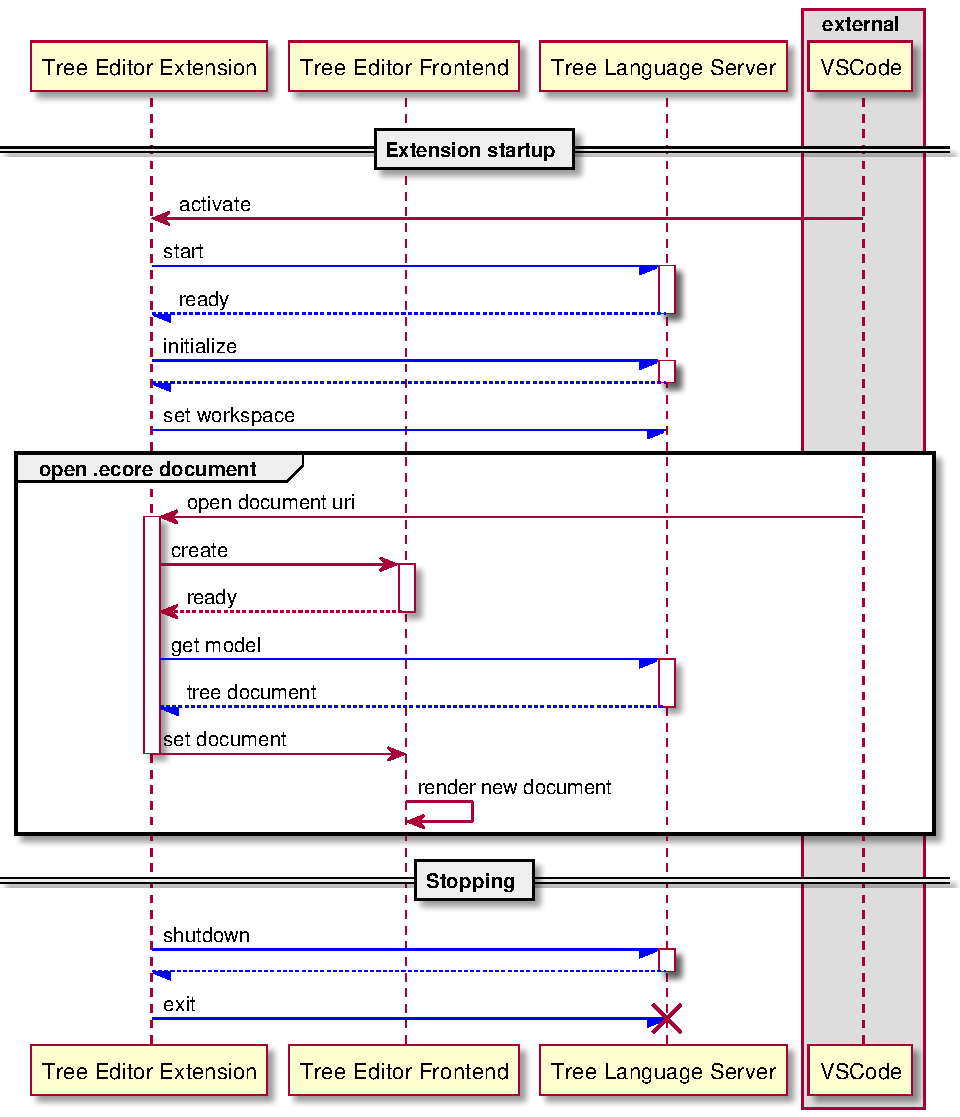
\includegraphics[width=\textwidth]{figures/plantuml/Protocol_startstop_sequence.pdf}
  \caption[Protocol Sequence Diagram of Start/Stop]{Sequence diagram for the protocol when starting and stopping the server. \bluearrowDesc}\label{fig:protocol-startstop}
\end{figure}

\begin{figure}[htbp]  % order of priority: h here, t top, b bottom, p page
  \centering
  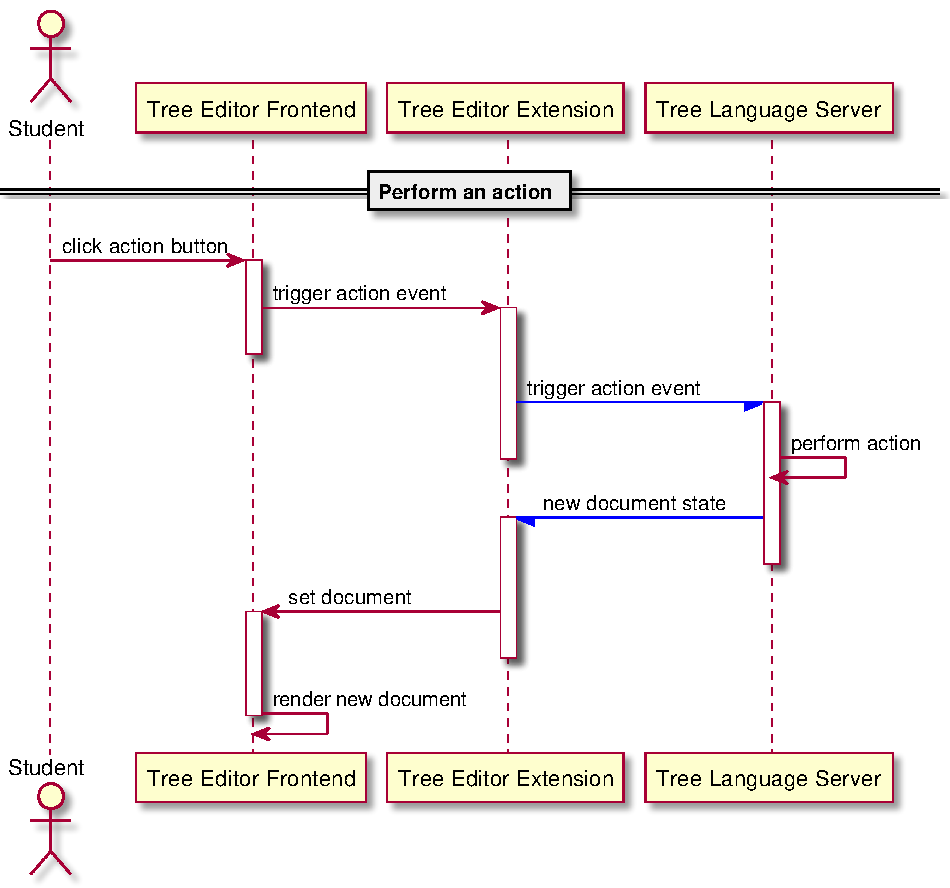
\includegraphics[width=\textwidth]{figures/plantuml/Protocol_action_sequence.pdf}
  \caption[Protocol Sequence Diagram of Action Triggering]{Sequence diagram for the protocol when triggering an action. \bluearrowDesc}\label{fig:protocol-action}
\end{figure}

\begin{figure}[htbp]  % order of priority: h here, t top, b bottom, p page
  \centering
  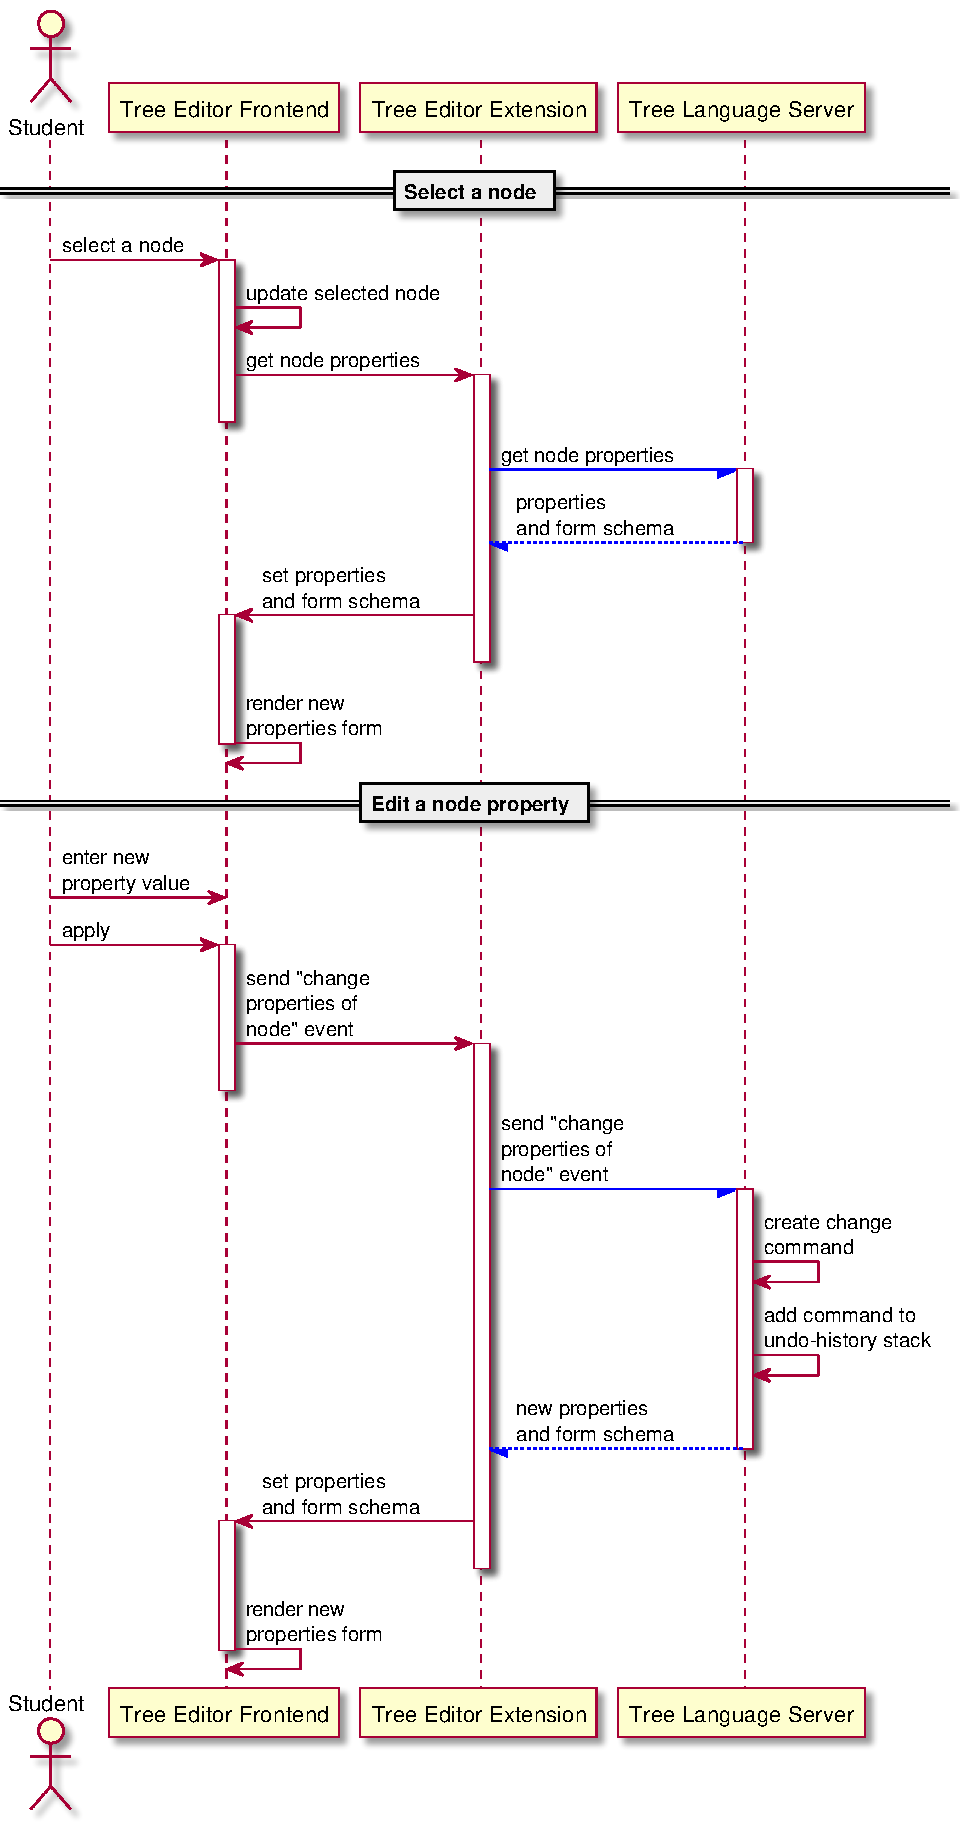
\includegraphics[width=\textwidth,height=\textheight,keepaspectratio]{figures/plantuml/Protocol_form_sequence.pdf}
  \caption[Protocol Sequence Diagram of Property Form]{Sequence diagram for the protocol when editing a node property. \bluearrowDesc}\label{fig:protocol-form}
\end{figure}

\begin{figure}[htbp]  % order of priority: h here, t top, b bottom, p page
  \centering
  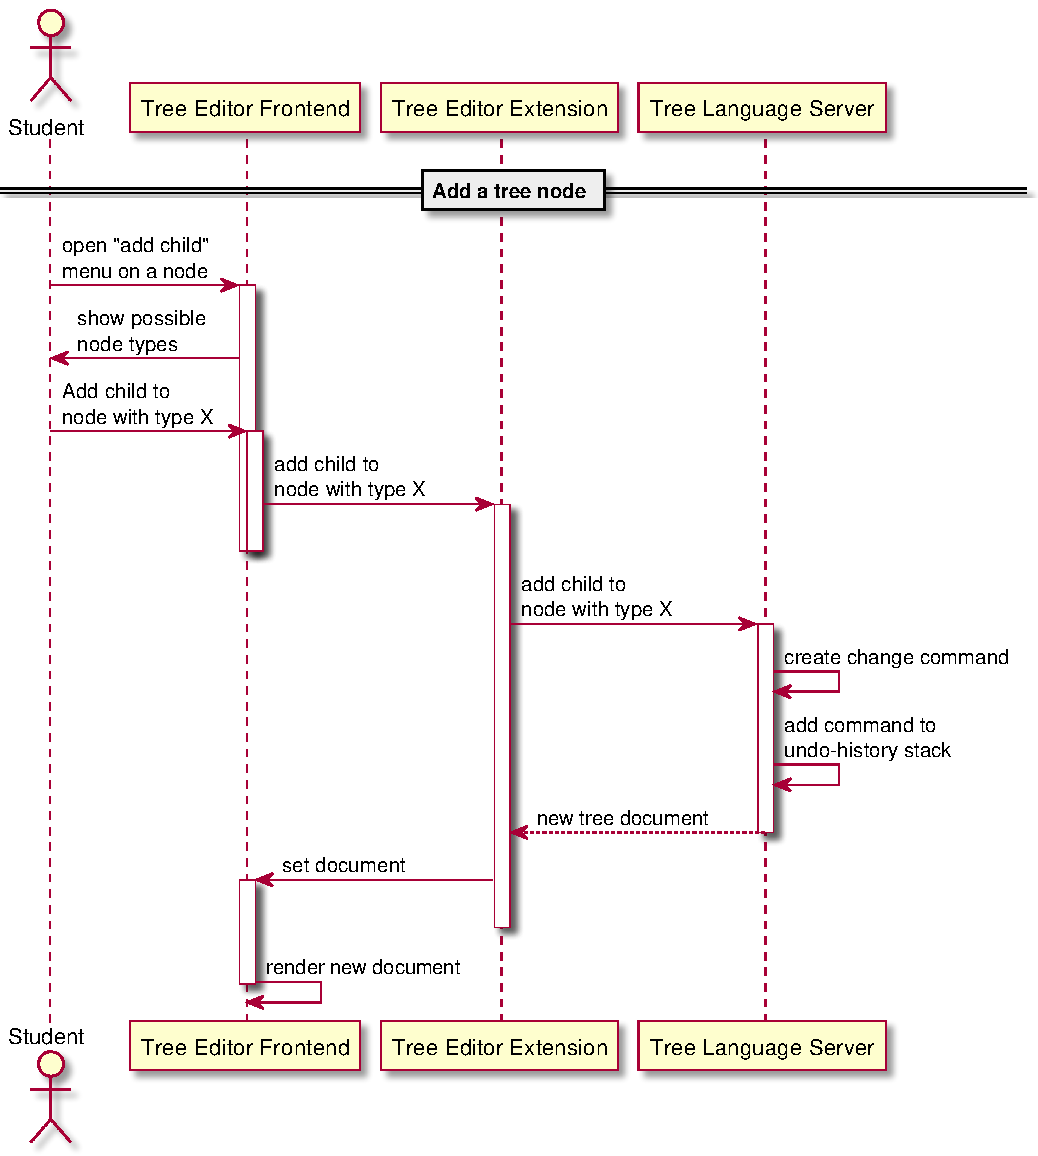
\includegraphics[width=\textwidth]{figures/plantuml/Protocol_changetree_sequence.pdf}
  \caption[Protocol Sequence Diagram of Tree Changes]{Sequence diagram for the protocol when adding a child node. \bluearrowDesc}\label{fig:protocol-changetree}
\end{figure}

\FloatBarrier
